\section{Definitions | relevant knowledge}\label{sec:02}
Adding pictures:
\begin{figure}[H]
	\begin{center}
		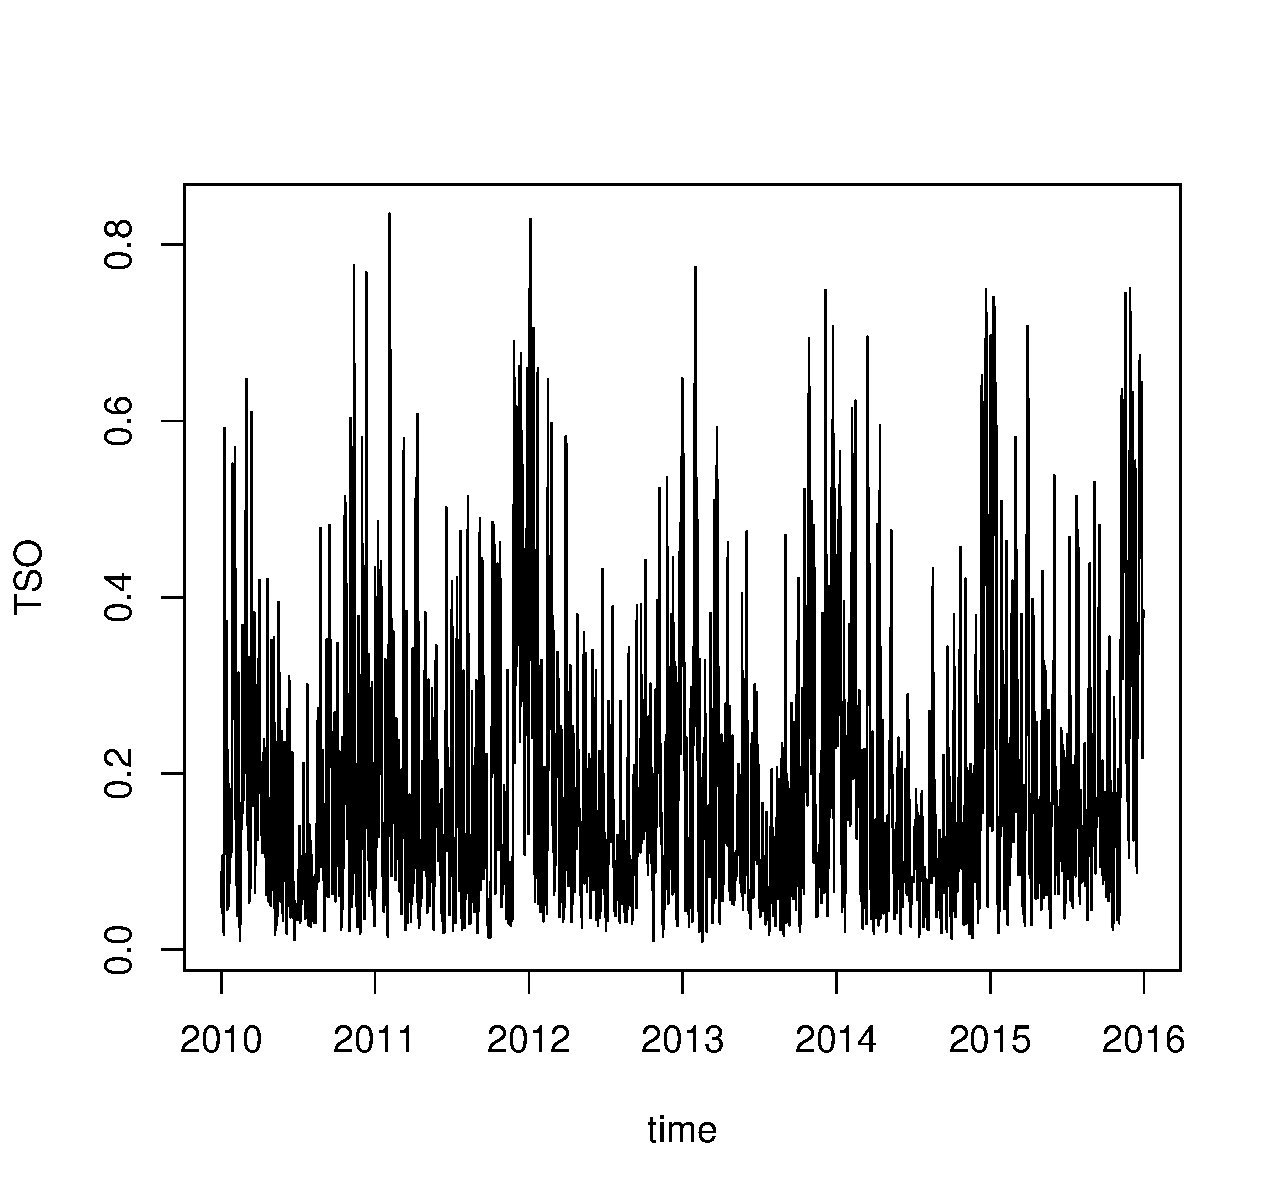
\includegraphics[scale=0.3]{Figures/TSO_ts}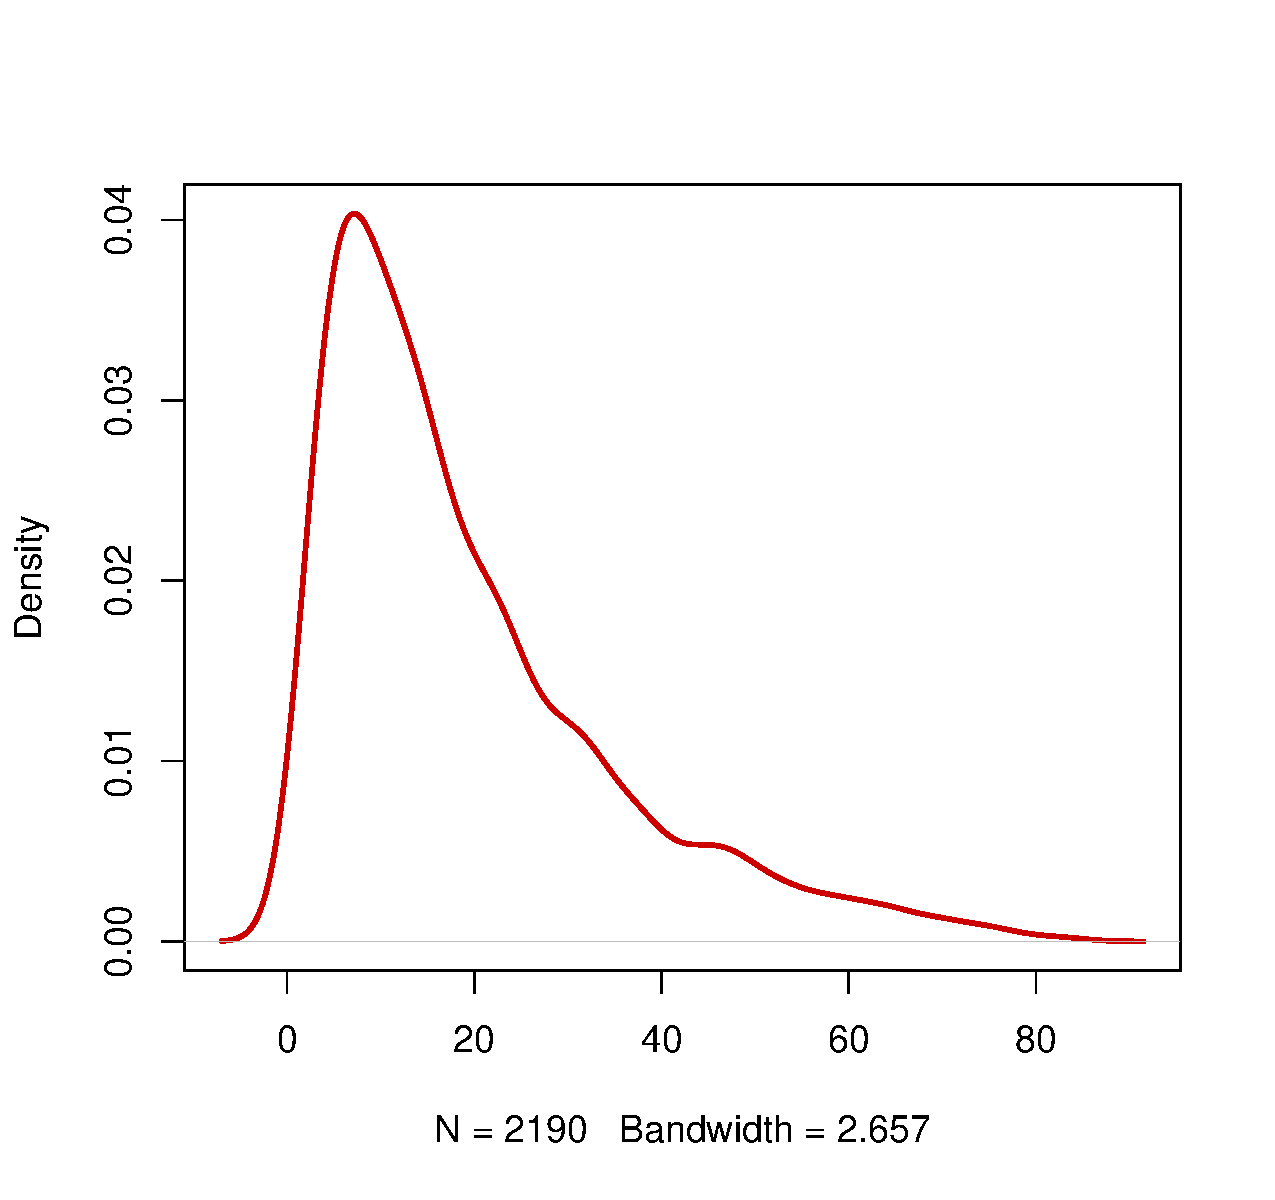
\includegraphics[scale=0.3]{Figures/TSO_dens}\\
		\caption{Time series (2010-2015) and its density of TSO data}
	\end{center}
\end{figure}

\newpage Adding graphs:
 \begin{figure}[H]
 	\begin{center}
 		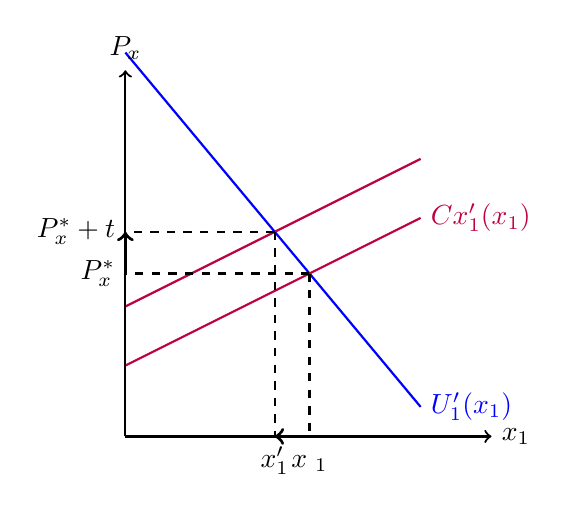
\begin{tikzpicture}[domain=0:5,scale=0.75,thick]
 		\usetikzlibrary{calc}                                %allows coordinate calculations.
 		\usetikzlibrary{decorations.pathreplacing}           %allows drawing curly braces.
 		
 		% Define linear parameters for supply and demand
 		\def\dint{6.5}      %Y-intercept for DEMAND.
 		\def\dslp{-1.2}     %Slope for DEMAND.
 		\def\sint{1.2}      %Y-intercept for SUPPLY.
 		\def\sintt{2.2}      %Y-intercept for SUPPLY.
 		\def\sslp{0.5}      %Slope for SUPPLY.
 		\def\tax{1.5}       %Excise (per-unit) tax
 		
 		% Define Supply and Demand Lines as equations of parameters defined above.
 		\def\demand{\x,{\dslp*\x+\dint}}
 		\def\supply{\x,{\sslp*\x+\sint}}
 		\def\demandtwo{\x,{\dslp*\x+\dint+\dsh}}
 		\def\supplytwo{\x,{\sslp*\x+\sint+\ssh}}
 		\def\supplyt{\x,{\sslp*\x+\sintt}}
 		
 		% Define coordinates.
 		\coordinate (ints) at ({(\sint-\dint)/(\dslp-\sslp)},{(\sint-\dint)/(\dslp-\sslp)*\sslp+\sint});
 		\coordinate (ep) at  (0,{(\sint-\dint)/(\dslp-\sslp)*\sslp+\sint});
 		\coordinate (eq) at  ({(\sint-\dint)/(\dslp-\sslp)},0);
 		\coordinate (dint) at (0,{\dint});
 		\coordinate (sint) at (0,{\sint});
 		\coordinate (teq) at  ({(\sint+\tax-\dint)/(\dslp-\sslp)},0); %quantity
 		\coordinate (tep) at  (0,{(\sint+\tax-\dint)/(\dslp-\sslp)*\sslp+\sint+\tax}); %price
 		\coordinate (tint) at  ({(\sint+\tax-\dint)/(\dslp-\sslp)},{(\sint+\tax-\dint)/(\dslp-\sslp)*\sslp+\sint+\tax}); %tax equilibrium
 		\coordinate (sep) at (0,{\sslp*(\sint+\tax-\dint)/(\dslp-\sslp)+\sint});
 		\coordinate (sen) at ({(\sint+\tax-\dint)/(\dslp-\sslp)},{\sslp*(\sint+\tax-\dint)/(\dslp-\sslp)+\sint});   
 		
 		% DEMAND
 		\draw[thick,color=blue] plot (\demand) node[right] {$U_1'(x_1)$};
 		
 		% SUPPLY
 		\draw[thick,color=purple] plot (\supply) node[right] {$Cx_1'(x_1)$};
 		\draw[thick,color=purple] plot (\supplyt) node[right] {}; 
 		\draw[very thick,<-] (4.3/1.7,0) -- (5.3/1.7,0);
 		\draw[very thick,<-] (0,0.5*4.3/1.7+2.2) -- (0,0.5*5.3/1.7+1.2);
 		% Draw axes, and dotted equilibrium lines.
 		\draw[->] (0,0) -- (6.2,0) node[right] {$x_1$};
 		\draw[->] (0,0) -- (0,6.2) node[above] {$P_x$};
 		\draw[dashed] (4.3/1.7,0.5*4.3/1.7+2.2) -- (0,0.5*4.3/1.7+2.2) node[left] {$P^{\ast}_x + t$};                  
 		\draw[dashed]  (5.3/1.7,0.5*5.3/1.7+1.2) -- (0,0.5*5.3/1.7+1.2) node[left] {$P^{\ast}_x$};
 		\draw[dashed]  (5.3/1.7,0.5*5.3/1.7+1.2) -- (5.3/1.7,0) node[below] {$x\phantom{'}_1$};                       
 		\draw[dashed]  (4.3/1.7,0.5*4.3/1.7+2.2) -- (4.3/1.7,0) node[below] {$x'_1$};      
 		
 		\end{tikzpicture}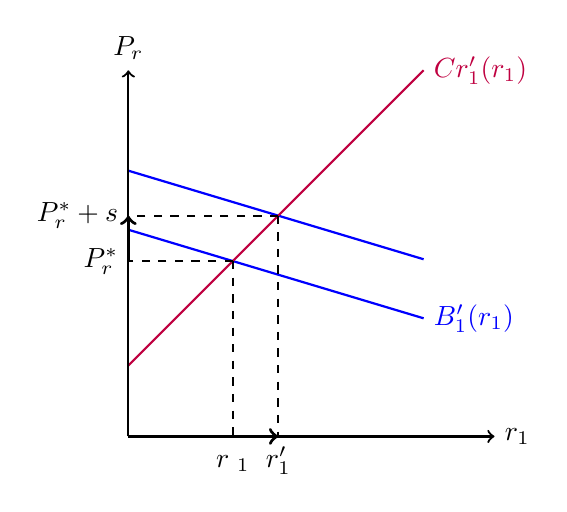
\begin{tikzpicture}[domain=0:5,scale=.75,thick]
 		\usetikzlibrary{calc}                                %allows coordinate calculations.
 		\usetikzlibrary{decorations.pathreplacing}           %allows drawing curly braces.
 		
 		% Define linear parameters for supply and demand
 		\def\dint{4.5}      %Y-intercept for DEMAND.
 		\def\dslp{-0.3}     %Slope for DEMAND.
 		\def\sint{1.2}      %Y-intercept for SUPPLY.
 		\def\dintt{3.5}      %Y-intercept for demand.
 		\def\sslp{1}         %Slope for SUPPLY.
 		\def\tax{1.5}       %Excise (per-unit) tax
 		
 		% Define Supply and Demand Lines as equations of parameters defined above.
 		\def\demand{\x,{\dslp*\x+\dint}}
 		\def\supply{\x,{\sslp*\x+\sint}}
 		\def\demandtwo{\x,{\dslp*\x+\dint+\dsh}}
 		\def\supplytwo{\x,{\sslp*\x+\sint+\ssh}}
 		\def\demandt{\x,{\dslp*\x+\dintt}}
 		
 		% Define coordinates.
 		\coordinate (ints) at ({(\sint-\dint)/(\dslp-\sslp)},{(\sint-\dint)/(\dslp-\sslp)*\sslp+\sint});
 		\coordinate (ep) at  (0,{(\sint-\dint)/(\dslp-\sslp)*\sslp+\sint});
 		\coordinate (eq) at  ({(\sint-\dint)/(\dslp-\sslp)},0);
 		\coordinate (dint) at (0,{\dint});
 		\coordinate (sint) at (0,{\sint});
 		\coordinate (teq) at  ({(\sint+\tax-\dint)/(\dslp-\sslp)},0); %quantity
 		\coordinate (tep) at  (0,{(\sint+\tax-\dint)/(\dslp-\sslp)*\sslp+\sint+\tax}); %price
 		\coordinate (tint) at  ({(\sint+\tax-\dint)/(\dslp-\sslp)},{(\sint+\tax-\dint)/(\dslp-\sslp)*\sslp+\sint+\tax}); %tax equilibrium
 		\coordinate (sep) at (0,{\sslp*(\sint+\tax-\dint)/(\dslp-\sslp)+\sint});
 		\coordinate (sen) at ({(\sint+\tax-\dint)/(\dslp-\sslp)},{\sslp*(\sint+\tax-\dint)/(\dslp-\sslp)+\sint});   
 		
 		% DEMAND
 		\draw[thick,color=blue] plot (\demand) node[right] {};
 		\draw[thick,color=blue] plot (\demandt) node[right] {$B_1'(r_1)$};      
 		% SUPPLY
 		\draw[thick,color=purple] plot (\supply) node[right] {$Cr_1'(r_1)$};
 		\draw[very thick,->] (2.3/1.3,0) -- (3.3/1.3,0);
 		\draw[very thick,->] (0,2.3/1.3+1.2) -- (0,3.3/1.3+1.2);
 		% Draw axes, and dotted equilibrium lines.
 		\draw[->] (0,0) -- (6.2,0) node[right] {$r_1$};
 		\draw[->] (0,0) -- (0,6.2) node[above] {$P_r$};
 		\draw[dashed] (3.3/1.3,3.3/1.3+1.2) -- (0,3.3/1.3+1.2) node[left] {$P^{\ast}_r + s$};                  
 		\draw[dashed]  (2.3/1.3,2.3/1.3+1.2) -- (0,2.3/1.3+1.2) node[left] {$P^{\ast}_r$};
 		\draw[dashed]  (3.3/1.3,3.3/1.3+1.2) -- (3.3/1.3,0) node[below] {$r'_1$};                       
 		\draw[dashed]  (2.3/1.3,2.3/1.3+1.2) -- (2.3/1.3,0) node[below] {$r\phantom{'}_1$}; 		
 		\end{tikzpicture}
 		\caption{Deposit refund policy.} \label{fig:DRP}
 	\end{center}
 \end{figure}
 
 